\section{方差}
\label{sec:rvm-variance}

两个游戏平均奖金都是$2$元，一个总是恰好给$2$元，另一个有一半机会一分不得、偶尔给$6$元。期望看不出这种差别。我们需要第二个数，衡量取值在均值周围散开的程度。上一节的平方误差已经给出了候选：用均值预测时的平均平方误差。本节把它定义为方差，说明存在条件、计算方法和它在平移、缩放下的变化，再由它得到与原变量同单位的标准差。

\subsection{定义}
\label{sec:rvm-variance-definition}

\paragraph{三个均值相同的游戏}
比较三张均值都是$2$的概率表：(a)恒取$2$；(b)以各$\tfrac12$的概率取$1$或$3$；(c)奖金表，以$\tfrac12,\tfrac13,\tfrac16$的概率取$0,3,6$。图~\ref{fig:rvm-same-mean}中三者的重心都在$2$，质量离重心的远近却明显不同。

怎样把“离重心多远”变成一个数？最直接的想法是平均偏差$\mathbb{E}[X-\mu]$，但由线性性它恒等于$\mathbb{E}[X]-\mu=0$：正负偏差正好抵消，这正是重心的定义。要避免抵消，可以取绝对值$\mathbb{E}\lvert X-\mu\rvert$，也可以取平方$\mathbb{E}[(X-\mu)^{2}]$。平方的好处是能展开：上一节的式~\eqref{eq:rvm-square-error}就是靠展开得到的，后面的计算公式、平移缩放规律以及第~\ref{chap:random-vectors}章和的方差都依赖这一点。

\begin{BookInlineFigure}
 \centering
 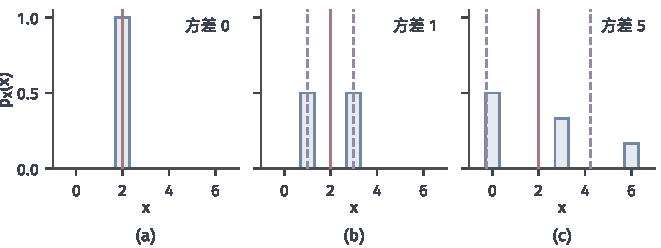
\includegraphics[width=112mm]{figures/07-probability/01-elementary-probability/matplotlib/rvm-same-mean/figure.pdf}
 \caption{三张均值都是$2$的概率表。(a)恒取$2$；(b)以各$\tfrac12$的概率取$1,3$；(c)奖金表。红线是均值，紫色虚线是均值加减标准差$\sqrt{\operatorname{Var}(X)}$。均值相同，方差依次为$0,1,5$。}
 \label{fig:rvm-same-mean}
\end{BookInlineFigure}

力学里也有同样的量。把单位质量按概率放在数轴上，到重心距离的平方乘质量再求和，就是这组质量绕重心的转动惯量。质量离重心越远，转动惯量越大，转动起来越费力。图~\ref{fig:rvm-variance-squares}把奖金表的每个偏差画成正方形，转动惯量就是这些正方形面积的概率加权和。这个类比在一处不完全对应：物理的转动惯量对任何有限质量分布都有限，而概率质量可以分布到无穷远，平方加权和可能是$+\infty$。

\begin{BookInlineFigure}
 \centering
 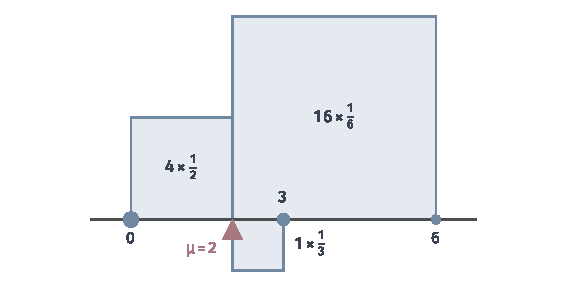
\includegraphics[width=96mm]{figures/07-probability/01-elementary-probability/matplotlib/rvm-variance-squares/figure.pdf}
 \caption{奖金表的方差是偏差平方的加权平均。三个取值到均值$\mu=2$的距离是$2,1,4$，对应正方形的面积是$4,1,16$（为避免重叠，$x=3$的正方形画在数轴下方），蓝点大小表示概率。按概率加权，$4\times\tfrac12+1\times\tfrac13+16\times\tfrac16=5$。}
 \label{fig:rvm-variance-squares}
\end{BookInlineFigure}

\paragraph{方差的定义}
平方的平均有意义，需要先有均值，并且平方的加权和有限。下面的定义把这两项要求都放在“$X^{2}$的期望有限”这一个条件里。

\begin{definition}[方差]
\label{def:rvm-variance}
设$\mathbb{E}[X^{2}]<\infty$，记$\mu=\mathbb{E}[X]$。称
\begin{equation}
 \operatorname{Var}(X)=\mathbb{E}\bigl[(X-\mu)^{2}\bigr]
 \label{eq:rvm-variance}
\end{equation}
为$X$的\term{方差}（variance），也记作$\sigma^{2}$或$\sigma_X^{2}$。
\end{definition}

条件$\mathbb{E}[X^{2}]<\infty$同时保证了均值有限和方差有限。由$(\lvert x\rvert-1)^{2}\geq0$得$\lvert x\rvert\leq\frac12(1+x^{2})$，所以
\[
 \mathbb{E}\lvert X\rvert\leq\tfrac12\bigl(1+\mathbb{E}[X^{2}]\bigr)<\infty .
\]
再由$(x-\mu)^{2}\leq2x^{2}+2\mu^{2}$，又得到
\[
 \mathbb{E}\bigl[(X-\mu)^{2}\bigr]\leq2\,\mathbb{E}[X^{2}]+2\mu^{2}<\infty .
\]这两步都是函数期望的比较，用到了保序性。

均值有限并不保证方差有限。密度$f_X(x)=2x^{-3}$（$x\geq1$）的均值是
\[
 \mathbb{E}[X]=\int_1^{\infty}x\cdot2x^{-3}\,\mathrm{d}x=2,
\]
但
\[
 \mathbb{E}[X^{2}]=\int_1^{\infty}x^{2}\cdot2x^{-3}\,\mathrm{d}x=\int_1^{\infty}\frac{2}{x}\,\mathrm{d}x=+\infty .
\]这时$(X-2)^{2}$是非负变量，它的期望按定义~\ref{def:rvm-expectation}等于$+\infty$，我们说$X$的方差无穷或不是有限的。远处的质量衰减得足以使一次方的力矩有限，却不足以使平方的力矩有限。

图~\ref{fig:rvm-same-mean}中三张表的方差分别是
\[
 0,\qquad (1-2)^{2}\cdot\tfrac12+(3-2)^{2}\cdot\tfrac12=1,\qquad 4\cdot\tfrac12+1\cdot\tfrac13+16\cdot\tfrac16=5 .
\]
方差的大小顺序与图中质量散开的程度一致。

\paragraph{方差为零}
方差是非负变量的期望，所以$\operatorname{Var}(X)\geq0$。方差为零意味着什么？它与“均值是某个数”不是一回事：图~\ref{fig:rvm-same-mean}中三张表的均值都是$2$，只有(a)的方差为零。下面说明方差为零恰好刻画了取值不变的变量。

\begin{theorem}[方差为零的变量]
\label{thm:rvm-zero-variance}
设$\mathbb{E}[X^{2}]<\infty$，$\mu=\mathbb{E}[X]$。
\begin{enumerate}
 \item 若$X$离散，则$\operatorname{Var}(X)=0$当且仅当$\mathbb{P}(X=\mu)=1$。
 \item 若$X$有密度，则$\operatorname{Var}(X)>0$。
\end{enumerate}
\end{theorem}

\begin{proof}
离散情形。$\operatorname{Var}(X)=\sum_i(x_i-\mu)^{2}p_X(x_i)$是非负项之和，它为零当且仅当每个$p_X(x_i)>0$的取值都满足$x_i=\mu$，即全部概率都在$\mu$上。

密度情形。取$\delta>0$，记$A_{\delta}=\{x:\lvert x-\mu\rvert\geq\delta\}$。在$A_{\delta}$上被积函数$(x-\mu)^{2}f_X(x)\geq\delta^{2}f_X(x)$，其余部分非负，所以
\[
 \operatorname{Var}(X)\geq\delta^{2}\int_{A_{\delta}}f_X(x)\,\mathrm{d}x=\delta^{2}\Bigl(1-\int_{\mu-\delta}^{\mu+\delta}f_X(x)\,\mathrm{d}x\Bigr) .
\]
$\delta\to0$时，长度趋于零的区间上的积分趋于零，所以对足够小的$\delta$，括号内大于$\tfrac12$，右边为正。
\end{proof}

这个结论把“数值恒定”说得很准确。方差为零的离散变量以概率一等于均值；若样本空间中还有概率为零的样本点，变量在那里可以取别的值，但这不影响任何概率和期望。有密度的变量把质量铺在一段长度上，不可能全部集中在一点，方差必然为正。对一般的随机变量，同样的刻画在第~\ref{chap:probability-spaces}章证明。

\subsection{计算}
\label{sec:rvm-variance-computation}

按定义计算方差需要两步：先求均值$\mu$，再对$(x-\mu)^{2}$加权求和或积分。对概率表与密度，两个公式分别是
\begin{equation}
 \operatorname{Var}(X)=\sum_{i}(x_i-\mu)^{2}p_X(x_i),\qquad
 \operatorname{Var}(X)=\int_{-\infty}^{\infty}(x-\mu)^{2}f_X(x)\,\mathrm{d}x .
 \label{eq:rvm-variance-formulas}
\end{equation}
它们是函数期望定理~\ref{thm:rvm-lotus}取$g(x)=(x-\mu)^{2}$的特殊情形。对密度$2x$，$\mu=\tfrac23$，展开被积函数后逐项积分，得到
\[
 \operatorname{Var}(X)=\int_0^12x\Bigl(x^{2}-\tfrac43x+\tfrac49\Bigr)\mathrm{d}x
 =2\Bigl(\tfrac14-\tfrac49+\tfrac29\Bigr)=\tfrac{1}{18} .
\]

把展开放在期望外面做，就得到一个通常更方便的公式，它只需要$\mathbb{E}[X]$与$\mathbb{E}[X^{2}]$。

\begin{theorem}[方差的展开式]
\label{thm:rvm-variance-shortcut}
设$\mathbb{E}[X^{2}]<\infty$，则
\begin{equation}
 \operatorname{Var}(X)=\mathbb{E}[X^{2}]-\bigl(\mathbb{E}[X]\bigr)^{2} .
 \label{eq:rvm-variance-shortcut}
\end{equation}
\end{theorem}

\begin{proof}
记$\mu=\mathbb{E}[X]$。$(X-\mu)^{2}=X^{2}-2\mu X+\mu^{2}$，右边三项都可积。由线性性，
\[
 \mathbb{E}\bigl[(X-\mu)^{2}\bigr]=\mathbb{E}[X^{2}]-2\mu\,\mathbb{E}[X]+\mu^{2}=\mathbb{E}[X^{2}]-\mu^{2} .
\]
\end{proof}

用展开式重算两个贯穿例子。奖金表的$\mathbb{E}[X^{2}]=9$，$\mathbb{E}[X]=2$，于是$\operatorname{Var}(X)=9-4=5$。密度$2x$的$\mathbb{E}[X^{2}]=\tfrac12$已在函数期望中算过，于是
\[
 \operatorname{Var}(X)=\tfrac12-\Bigl(\tfrac23\Bigr)^{2}=\tfrac{9-8}{18}=\tfrac{1}{18} .
\]
两个结果都与按定义计算的一致。由于方差非负，式~\eqref{eq:rvm-variance-shortcut}也重新给出了$\mathbb{E}[X^{2}]\geq(\mathbb{E}[X])^{2}$，这是\term{Jensen不等式}在$f(x)=x^{2}$时的情形。

把式~\eqref{eq:rvm-variance-shortcut}与上一节的式~\eqref{eq:rvm-square-error}放在一起，得到对任意常数$c$成立的分解
\begin{equation}
 \mathbb{E}\bigl[(X-c)^{2}\bigr]=\operatorname{Var}(X)+(\mathbb{E}[X]-c)^{2} .
 \label{eq:rvm-parallel-axis}
\end{equation}
用转动惯量的语言，它说绕任一点$c$的转动惯量等于绕重心的转动惯量加上重心到$c$的距离平方，这是力学中的平行轴定理。图~\ref{fig:rvm-error-curves}(a)中抛物线的最低值$5$就是奖金表的方差。

\paragraph{两种算法的比较}
按定义计算时，每一项$(x_i-\mu)^{2}$都非负，结果天然非负，但必须先算出$\mu$再回头处理每个取值；展开式只需要分别累计$x_i$与$x_i^{2}$的加权和，一遍就能完成，求积分时常常也更简单。代价在于展开式是两个可能很大的数相减。

把奖金表的每个取值都加上$10^{8}$，方差仍是$5$。用双精度浮点数计算，$\mathbb{E}[X^{2}]$与$(\mathbb{E}[X])^{2}$都约为$10^{16}$，而这个量级上相邻两个浮点数相差$2$，两数之差只剩下很少的有效数字。实际计算得到$4$；平移量增大到$10^{9}$时，展开式给出$0$。按定义先减去均值再平方，两种平移下得到的都是$5$。所以手算或求解析式时常用展开式，而均值相对波动很大的数值计算应先中心化。

\subsection{平移与缩放}
\label{sec:rvm-variance-affine}

参加一次奖金游戏要付$2$元，净收益是$X-2$；把赌注加倍，奖金变成$2X$；站在庄家一边，收益是$-X$。这些变量的方差与$X$的方差有什么关系？它们都是$aX+b$的形式，答案由中心化后的偏差决定。

\begin{theorem}[方差的平移与缩放]
\label{thm:rvm-variance-affine}
设$\mathbb{E}[X^{2}]<\infty$，$a,b$为实数。则$\mathbb{E}[(aX+b)^{2}]<\infty$，且
\begin{equation}
 \mathbb{E}[aX+b]=a\,\mathbb{E}[X]+b,\qquad \operatorname{Var}(aX+b)=a^{2}\operatorname{Var}(X) .
 \label{eq:rvm-variance-affine}
\end{equation}
\end{theorem}

\begin{proof}
$(ax+b)^{2}\leq2a^{2}x^{2}+2b^{2}$，所以$(aX+b)^{2}$可积。均值的公式是线性性。记$\mu=\mathbb{E}[X]$，新变量的偏差是
\[
 (aX+b)-(a\mu+b)=a(X-\mu),
\]
平移量$b$在相减时消去。平方后取期望，得到
\[
 \operatorname{Var}(aX+b)=\mathbb{E}\bigl[a^{2}(X-\mu)^{2}\bigr]=a^{2}\operatorname{Var}(X) .
\]
\end{proof}

平移整体移动所有取值，不改变它们之间的距离，所以方差不变；缩放把每个偏差乘以$a$，平方后方差乘以$a^{2}$。图~\ref{fig:rvm-shift-scale}画出了奖金表的三个变换：$X-2$的均值是$0$，方差仍是$5$；$2X$的均值是$4$，方差是$4\times5=20$；$-X$把分布左右翻转，均值是$-2$，方差仍是$5$，因为$(-1)^{2}=1$。

\begin{BookInlineFigure}
 \centering
 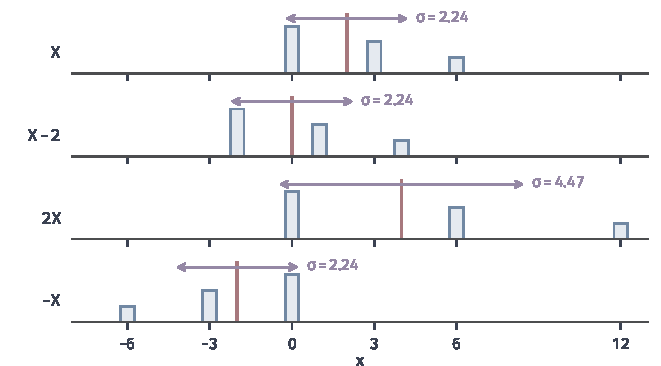
\includegraphics[width=112mm]{figures/07-probability/01-elementary-probability/matplotlib/rvm-shift-scale/figure.pdf}
 \caption{奖金表$X$及其平移、缩放与反射。红线是均值，紫色双箭头是均值加减一个标准差。$X-2$整体左移，宽度不变；$2X$的取值间距加倍，标准差从$2.24$变为$4.47$；$-X$左右翻转，标准差不变。}
 \label{fig:rvm-shift-scale}
\end{BookInlineFigure}

两个特殊情形值得核对。$a=0$时$aX+b$是常数$b$，公式给出方差$0$，与定理~\ref{thm:rvm-zero-variance}一致。$a<0$时缩放同时带来反射，方差只与$\lvert a\rvert$有关，波动的大小不区分方向。

式~\eqref{eq:rvm-variance-affine}只处理一个变量的线性函数。两个不同变量相加时，偏差的平方会产生交叉项。例如$X+X=2X$的方差是$4\operatorname{Var}(X)=20$，而不是$\operatorname{Var}(X)+\operatorname{Var}(X)=10$，多出的$10$正来自交叉项$2\,\mathbb{E}[(X-\mu)(X-\mu)]$。一般的和的方差由协方差描述，在第~\ref{chap:random-vectors}章计算。

\subsection{标准差与标准化}
\label{sec:rvm-standardization}

奖金以元为单位，方差的单位却是“平方元”，$5$平方元很难与$2$元的均值直接比较。开平方就回到原来的单位。

\begin{definition}[标准差]
\label{def:rvm-std}
设$\mathbb{E}[X^{2}]<\infty$。称方差的非负平方根
\begin{equation}
 \sigma_X=\sqrt{\operatorname{Var}(X)}
 \label{eq:rvm-std}
\end{equation}
为$X$的\term{标准差}（standard deviation）。
\end{definition}

奖金表的标准差是$\sqrt5\approx2.24$元，密度$2x$的标准差是$1/\sqrt{18}\approx0.236$。由式~\eqref{eq:rvm-variance-affine}，$\sigma_{aX+b}=\lvert a\rvert\sigma_X$：标准差与变量同步缩放，单位换算时直接乘以换算系数。标准差可以解读为偏差的典型大小，但它是平方平均的平方根，不是平均偏差：奖金表的$\mathbb{E}\lvert X-2\rvert=2$，比$\sqrt5$小，因为平方放大了远处那个偏差$4$的分量。偏离均值超过若干个标准差的概率有多大，要用第~\ref{chap:tail-probabilities}章的尾概率工具估计。

\paragraph{标准化}
均值和标准差分别给出位置和尺度。把它们都除去，就得到一个与单位和位置无关的变量，便于比较不同量纲的随机量，或者描述“偏离均值多少个标准差”。

\begin{definition}[标准化]
\label{def:rvm-standardize}
设$\mathbb{E}[X^{2}]<\infty$且$\sigma_X>0$，$\mu=\mathbb{E}[X]$。称
\begin{equation}
 Z=\frac{X-\mu}{\sigma_X}
 \label{eq:rvm-standardize}
\end{equation}
为$X$的\term{标准化}（standardization）。由式~\eqref{eq:rvm-variance-affine}取$a=1/\sigma_X$，$b=-\mu/\sigma_X$，得$\mathbb{E}[Z]=0$，$\operatorname{Var}(Z)=1$。
\end{definition}

两个条件都不能少。方差必须有限，否则没有可除的尺度；方差必须为正，常数变量没有波动，无法放大成方差为一的变量。

对奖金表，$Z=(X-2)/\sqrt5$以概率$\tfrac12,\tfrac13,\tfrac16$取
\[
 -\tfrac{2}{\sqrt5}\approx-0.89,\qquad \tfrac{1}{\sqrt5}\approx0.45,\qquad \tfrac{4}{\sqrt5}\approx1.79 .
\]
直接核对均值与方差：
\[
 \mathbb{E}[Z]=\tfrac{1}{\sqrt5}\bigl(-1+\tfrac13+\tfrac23\bigr)=0,\qquad
 \mathbb{E}[Z^{2}]=\tfrac15\bigl(2+\tfrac13+\tfrac83\bigr)=1 .
\]对密度$2x$，$Z=\sqrt{18}\,(X-\tfrac23)$的取值范围是$(-2\sqrt2,\sqrt2)$。

\begin{BookInlineFigure}
 \centering
 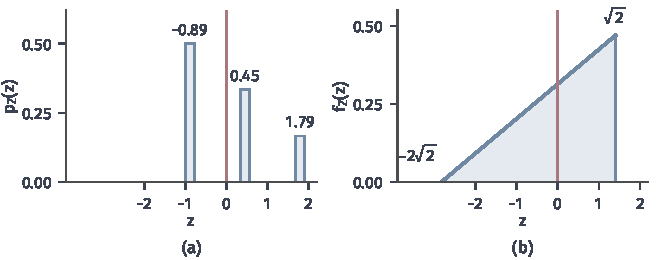
\includegraphics[width=112mm]{figures/07-probability/01-elementary-probability/matplotlib/rvm-standardized/figure.pdf}
 \caption{标准化不改变分布的形状。(a)奖金表标准化后的概率表；(b)密度$2x$标准化后的密度，支撑为$(-2\sqrt2,\sqrt2)$。两者均值都是$0$（红线）、方差都是$1$，但一个是右侧拖尾的三点分布，一个是向右上升的三角形，都不是钟形。}
 \label{fig:rvm-standardized}
\end{BookInlineFigure}

图~\ref{fig:rvm-standardized}说明标准化只做平移和正的缩放，概率表的相对位置和密度的形状都原样保留。均值为零、方差为一并不意味着分布接近某个特定形状，标准化后的奖金仍然只取三个值，仍然向右偏。许多独立小扰动之和标准化后才会接近钟形，那是第~\ref{chap:central-limit-theorem}章的定理，需要独立性和求和，不是标准化本身的效果。
